\documentclass[journal]{IEEEtran}

\usepackage{cite}
\usepackage{amsmath,amssymb,amsfonts,amsthm}
\usepackage{algorithm}
\usepackage{algorithmic}
\usepackage{graphicx}
\usepackage{booktabs}
\usepackage{array}
\usepackage{placeins}
\usepackage{url}
\usepackage[hidelinks]{hyperref}

\emergencystretch=1.2em
\renewcommand{\dbltopfraction}{0.82}
\renewcommand{\dblfloatpagefraction}{0.75}
\renewcommand{\textfraction}{0.08}
\setlength{\dbltextfloatsep}{7pt plus 2pt minus 2pt}
\setlength{\textfloatsep}{8pt plus 2pt minus 2pt}
\setlength{\abovecaptionskip}{3pt}

\newtheorem{proposition}{Proposition}

\hyphenation{op-tical net-works semi-conduc-tor spectral clustering bipartite feedback multi-modal control-ler eigengap stability}

% TODO(PERSONAL_INFO): Update target journal if not IEEE Transactions on Cybernetics, and replace [Author Surname]
\markboth{SUBMITTED TO IEEE TRANSACTIONS ON CYBERNETICS}{[Author Surname]: Closed-Loop PI Feedback and Bipartite Spectral Control}

\begin{document}

\title{Closed-Loop Proportional--Integral Feedback and Linear-Time Bipartite Spectral Control for Fault-Tolerant Multi-Modal Clustering}

% TODO(PERSONAL_INFO): Replace bracketed author name(s), affiliation, email, ORCID, and optional grant number before submission.
\author{[Author Full Name]%
\thanks{This work was supported in part by [Grant / Funding Agency, if applicable, or delete this sentence].}%
\thanks{[Author Full Name] is with the [Department / School], [University / Institution], [City] [Postal Code], [Country] (e-mail: [author@institution.edu]; ORCID: [0000-0000-0000-0000]). Source code, reproducible Colab notebooks, and benchmark archives are publicly available at \url{https://github.com/dashitongzhi/CL-VSSC}.}}

\maketitle

\begin{abstract}
Multi-modal representation learning separates shared biological structure from nuisance variance before spectral clustering. Existing consensus graph learners and deep encoders mostly run in open loop: view weights lack partition feedback, eigengaps stay unregulated, and $\mathcal{O}(n^3)$ eigendecompositions fail on $10^5$-sample cohorts. We formulate multi-modal clustering as a discrete-time closed-loop feedback system (\textbf{CL-VSSC}) paired with a linear-time bipartite landmark controller (\textbf{CL-VSSC-Anchor}, $\mathcal{O}(nm^2+ndr)$). An orthogonal Stiefel plant couples with a dual Ky Fan eigengap controller and a damped simplex proportional--integral (PI) controller (with Null-SNR and double-centered Anchor-Local modes) under Input-to-State Stability (ISS) and Davis--Kahan bounds. Across $1{,}560$ TCGA three-modality stress runs ($\sigma\le 4.0$, up to $60\%$ dropout), Smooth PI lowers faulty weights to $0.012$ (vs.\ $0.190$ MCGC, $0.264$ Seurat-WNN, $0.319$ Attention-MOAE; BH-FDR $q=1.46\times 10^{-11}$). Null-SNR calibration cuts leakage to $0.002$ and raises mean fault ARI by $+0.103$ ($0.484 \rightarrow 0.587$; $0.796$ on mRNA/miRNA faults, $q \le 6.19\times 10^{-4}$). On the NeurIPS \texttt{GSE194122} CITE-seq atlas ($90{,}261$ cells, $45$ types), CL-VSSC-Anchor accelerates $10{,}000$-cell A100 runtime $20.3\times$ ($4.60\text{ s}$ vs.\ $93.58\text{ s}$), cuts VRAM $13.3\times$ ($603$ vs.\ $8{,}002\text{ MB}$), processes all $90{,}261$ cells in $16.57\text{ s}$ ($5{,}295\text{ MB}$; $21.71\text{ s}$ Local PI on L4), and leads Protein-ADT fault ARI ($\sigma=3.0$: $0.169$ vs.\ $0.051$ Attention-MOAE). Extended A100-80GB validation maps $536$ $(K_p,K_i,\delta_{\mathrm{dz}})$ stability points, follows $\mathcal{O}(N^{0.996})$ VRAM scaling to $300{,}000$ cells ($52.98\text{--}53.56\text{ s}$), and achieves $7$-iteration ($3.82\text{--}6.03\text{ s}$) step-fault recovery at $N=200{,}000$.
\end{abstract}

\begin{IEEEkeywords}
Closed-loop feedback control, PI mirror descent, input-to-state stability, bipartite spectral clustering, fault tolerance, CITE-seq.
\end{IEEEkeywords}

\section{Introduction}

\IEEEPARstart{A}{utonomous} integration of heterogeneous multi-modal measurements must fuse complementary views while isolating degraded sensors and batch perturbations \cite{rappoport2018multi,astrom2008feedback}. Joint--individual factorization models \cite{lock2013jive}, graph diffusion pipelines \cite{wang2014snf,rappoport2019nemo}, consensus graph learners \cite{nie2016clr,zhan2018mvgl,zhan2019mcgc}, and multimodal deep encoders \cite{yang2021subtypegan,moon2022moma,gayoso2021totalvi} have achieved strong empirical performance under curated conditions. Drawing on feedback systems and online feedback optimization (OFO) principles \cite{astrom2008feedback,hauswirth2024ofo}, viewing joint variable separation, view weighting, and spectral partitioning as a closed dynamical loop exposes three fundamental control bottlenecks:
\begin{enumerate}
    \item \emph{Open-loop fault leakage and steady-state offset}: When view weights rely solely on heuristic graph discrepancies \cite{zhan2019mcgc} or amortized encoders \cite{moon2022moma}, corrupted channels inject spurious edges directly into the fused graph. Memoryless proportional updates likewise plateau at persistent nonzero leakage under sustained sensor noise \cite{astrom2008feedback}.
    \item \emph{Unregulated eigengaps and dead-zone miscalibration}: Post-hoc spectral clustering \cite{ng2001spectral,vonluxburg2007tutorial} leaves small normalized Laplacian eigengaps $\Delta\lambda_c$ vulnerable to perturbation \cite{davis1970rotation}, whereas arbitrary dead-zone thresholds blunt sensitivity to moderate SNR disparities.
    \item \emph{Cubic computational scaling}: Dense $n \times n$ graph construction and eigendecomposition demand $\mathcal{O}(n^3)$ time and $\mathcal{O}(n^2)$ memory, precluding large single-cell atlases unless landmark bipartite structures \cite{fowlkes2004nystrom,cai2015lsc,kang2020lmvsc,xia2023tbgl,huang2023fastmice} are regulated directly inside the feedback loop.
\end{enumerate}

To resolve all three challenges systematically, we develop \textbf{CL-VSSC} and its linear-time extension \textbf{CL-VSSC-Anchor} (Fig.~\ref{fig:p2_control_loop}), with four main contributions:
\begin{itemize}
    \item \textbf{Closed-loop dual spectral--PI architecture}: Combines a Stiefel-manifold orthogonal plant \cite{edelman1998geometry} with a dual integral Ky Fan trace controller ($\mu$) and a damped simplex PI mirror-descent controller \cite{beck2003mirror} ($\delta_{\mathrm{dz}} = 0$ Smooth PI, Null-SNR baseline normalization, and double-centered Anchor-Local PI).
    \item \textbf{Three formal control propositions}: Establishes exact $\mathcal{O}(nm^2)$ Gram eigendecomposition equivalence (Proposition~1), $(1+\kappa_I)/\tau$ exponential fault attenuation and dead-zone blocking analysis (Proposition~2), and Input-to-State Stability (ISS) \cite{sontag1989smooth,sontag2008iss} with a Davis--Kahan $\sin\Theta$ spectral perturbation bound \cite{davis1970rotation} (Proposition~3).
    \item \textbf{Three-modality stress \& 90k single-cell scaling}: Achieves severe-fault attenuation ($0.012$ Smooth PI, $0.002$ Null-SNR PI) across $1{,}560$ TCGA runs plus $20.3\times$ speedup and $13.3\times$ memory savings on the $90{,}261$-cell NeurIPS CITE-seq bone marrow atlas \cite{luecken2021sandbox,stoeckius2017citeseq,hao2021seuratv4}.
    \item \textbf{Empirical control-gain Pareto and stability phase mapping}: Quantifies clean compactness against fault resilience across $(\kappa_I, \tau)$, $\mu_{\max}$, and $m$, maps $536$ $(K_p, K_i, \delta_{\mathrm{dz}})$ stability regimes, and verifies $300{,}000$-cell scaling and $200{,}000$-cell step-fault self-healing.
\end{itemize}

\begin{figure*}[t]
    \centering
    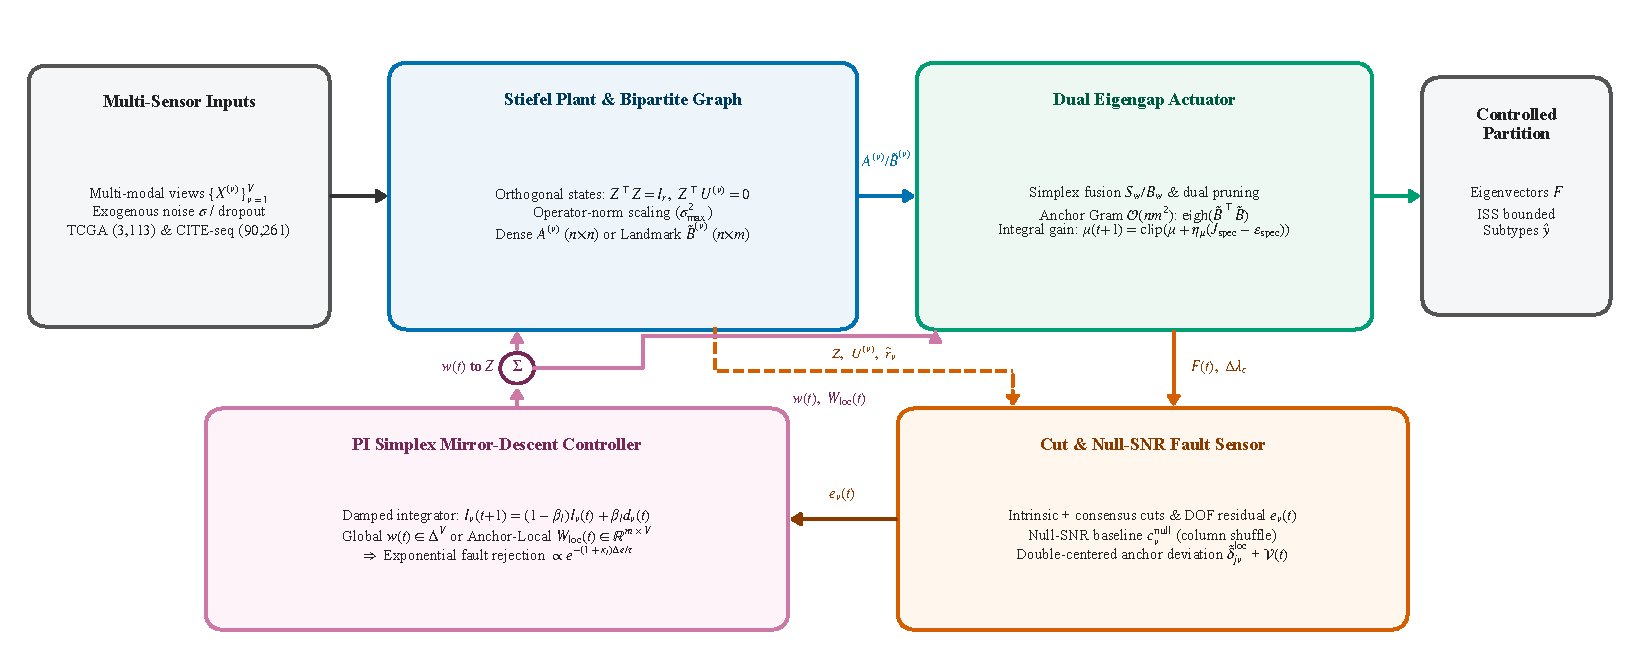
\includegraphics[width=0.95\textwidth]{figures/p2_fig1_control_loop.pdf}
    \caption{Closed-loop feedback control architecture of CL-VSSC and CL-VSSC-Anchor. The Stiefel orthogonal plant generates dense ($A^{(v)}$) or bipartite landmark ($\tilde{B}^{(v)}$) representations regulated by a dual integral eigengap controller $\mu(t)$. An observable cut and Null-SNR fault sensor feeds back through a damped PI simplex controller ($w(t)$ or $W_{\mathrm{loc}}(t)$) to reject corrupted sensors.}
    \label{fig:p2_control_loop}
\end{figure*}

\section{Related Work}

\subsection{Variable Separation, Consensus Graphs, and Feedback Control}
Joint--individual separation architectures decouple shared biological variance from modality-specific noise \cite{lock2013jive}. In graph clustering, CLR \cite{nie2016clr}, MVGL \cite{zhan2018mvgl}, and MCGC \cite{zhan2019mcgc} constrain Laplacian rank through Ky Fan's theorem \cite{fan1949theorem}, yet weight modalities using heuristic inverse graph discrepancy without integral memory or partition feedback. Concurrently, deep attention models such as MOMA \cite{moon2022moma} and \texttt{Subtype-\allowbreak GAN} \cite{yang2021subtypegan} learn static sample weights that can lock onto high-variance noisy assays. Extending the view of iterative optimizers as robust feedback controllers \cite{astrom2008feedback,sontag2008iss,hauswirth2024ofo} to multi-view graph fusion, our companion paper \cite{cao2026mivscl} develops a mask-aware Stiefel--graph solver for missing-block imputation on clinical TCGA cohorts. Starting from that Stiefel core, this work introduces four control-theoretic extensions: Null-SNR calibration, linear-time bipartite landmark control with double-centered Anchor-Local PI (\texttt{CL-\allowbreak VSSC-\allowbreak Anchor}), ISS and Davis--Kahan bounds, and 1,560-run stress plus 90,261-cell CITE-seq validation.

\subsection{Large-Scale Anchor Spectral Clustering and CITE-seq}
To avoid $\mathcal{O}(n^3)$ scaling, Nystr\"om approximations \cite{fowlkes2004nystrom}, LSC \cite{cai2015lsc}, LMVSC \cite{kang2020lmvsc}, tensorized bipartite fusion \cite{xia2023tbgl}, and FastMICE \cite{huang2023fastmice} build compact bipartite cell--anchor graphs in open loop. In single-cell CITE-seq \cite{stoeckius2017citeseq}, \texttt{Seurat-\allowbreak WNN} \cite{hao2021seuratv4} assigns cell weights from local k-NN prediction ratios, whereas totalVI \cite{gayoso2021totalvi} uses variational autoencoders. \texttt{CL-\allowbreak VSSC-\allowbreak Anchor} differs by running closed-loop PI weighting and dual spectral pruning directly on the sparse $n \times m$ bipartite graph.

\section{Closed-Loop Control Methodology and Stability}

Given $V$ assays $\{X^{(v)} \in \mathbb{R}^{n \times d_v}\}_{v=1}^V$ standardized to unit variance and scaled by $\sqrt{d_v}$, let $\Delta^V$ denote the $V$-dimensional simplex and $c$ be the cluster count.

\subsection{Orthogonal Plant and Dual Eigengap Actuator}
At iteration $t$, shared state $Z(t) \in \mathbb{R}^{n \times r}$ and specific factors $U^{(v)}(t) \in \mathbb{R}^{n \times r_v}$ evolve on mutually orthogonal Stiefel manifolds ($Z^\top Z = I_r$, $Z^\top U^{(v)} = 0$) through polar retraction $\Pi_{\mathcal{S}}$ \cite{edelman1998geometry}. Normalizing each view by its squared operator norm $s_v^2 = \sigma_{\max}^2(X^{(v)}) + 10^{-8}$ gives the scale-invariant shared update:
\begin{equation}
\begin{aligned}
G_Z(t) &= \lambda_Z \mathcal{T}_S(Z(t)) + \sum_{v=1}^V \frac{w_v(t)}{s_v^2} X_{\mathrm{sh}}^{(v)}(t) P^{(v)}(t)^\top, \\
Z(t+1) &= \Pi_{\mathcal{S}}\!\left((1-\eta_Z) Z(t) + \eta_Z \Pi_{\mathcal{S}}(G_Z(t))\right),
\end{aligned}
\label{eq:p2_plant}
\end{equation}
where $X_{\mathrm{sh}}^{(v)} = X^{(v)} - U^{(v)} Q^{(v)}$ and $\mathcal{T}_S$ applies normalized affinity propagation. Using softly denoised features $\bar{X}_{\mathrm{sh}}^{(v)} = X^{(v)} - \beta_u U^{(v)} Q^{(v)}$ ($\beta_u = 0.35$), dense mode builds self-tuning k-NN affinities $A^{(v)} \in \mathbb{R}^{n \times n}$ \cite{vonluxburg2007tutorial} and fuses $S_{\mathrm{w}}(t) = \sum_v w_v(t) A^{(v)}$. For Laplacian $L(S)$ with bottom-$c$ eigenvectors $F(t)$, Ky Fan's trace violation $J_{\mathrm{spec}} = \operatorname{Tr}(F^\top L(S) F)$ \cite{fan1949theorem} drives cross-cluster edge pruning ($H_{ij} = \|\hat{f}_i - \hat{f}_j\|_2^2$) and clipped dual gain integration ($t \ge t_{\mathrm{warm}}$):
\begin{equation}
\begin{aligned}
\tilde{S}_{\mathrm{tgt}}(t) &= \operatorname{clip}_+\!\left(S_{\mathrm{w}}(t) - \frac{0.14\,\mu(t)}{k} H(t)\right), \\
\mu(t+1) &= \operatorname{clip}\!\left(\mu(t) + \eta_\mu(J_{\mathrm{spec}}(t+1) - \epsilon_{\mathrm{spec}}),\; 0,\; \mu_{\max}\right),
\end{aligned}
\label{eq:p2_dual}
\end{equation}
followed by symmetric row normalization and EMA blending $S(t+1) = (1-\eta_S)S(t) + \eta_S \hat{S}_{\mathrm{tgt}}(t)$.

\begin{table*}[t]
\centering
\caption{Closed-Loop Controller and Sensor Ablation on 10 TCGA Cohorts and $\sigma=4.0$ Multi-Modal Sensor Faults}
\label{tab:p2_ablation}
\scriptsize
\renewcommand{\arraystretch}{1.14}
\setlength{\tabcolsep}{3.0pt}
\begin{tabular}{lcccccccc}
\toprule
Variant & \shortstack{Clean Sig.\\($p_{\mathrm{perm}}{<}0.05$)} & \shortstack{Clean Mean\\$-\log_{10}p_{\mathrm{perm}}$} & \shortstack{Clean Med.\\$-\log_{10}p_{\mathrm{perm}}$} & \shortstack{Clean\\Silhouette} & \shortstack{$k$-Sweep\\(/40)} & \shortstack{BIC Fault\\$w_{\mathrm{mRNA}}$} & \shortstack{Fault Mean\\$w_{\mathrm{corr}}$} & \shortstack{Fault ARI\\(36 runs)} \\
\midrule
CL-VSSC (Smooth PI) & \textbf{5/10} & 1.299 & 1.248 & 0.509 & \textbf{23/40} & 0.011 & 0.012 & 0.484 \\
CL-VSSC (Null-SNR) & 3/10 & 1.223 & 0.882 & \textbf{0.516} & 21/40 & \textbf{0.001} & \textbf{0.002} & \textbf{0.587} \\
CL-VSSC (DZ-PI) & 4/10 & 1.183 & 0.845 & 0.499 & 20/40 & 0.021 & 0.024 & 0.467 \\
P-only & 4/10 & 1.218 & 0.809 & 0.499 & --- & 0.031 & --- & --- \\
w/o Feedback & 4/10 & 1.534 & 1.220 & 0.497 & --- & 0.333 & 0.333 & 0.453 \\
w/o SpecCtrl & 4/10 & 1.205 & 0.887 & 0.481 & --- & --- & --- & --- \\
\bottomrule
\end{tabular}
\end{table*}


\begin{figure*}[t]
    \centering
    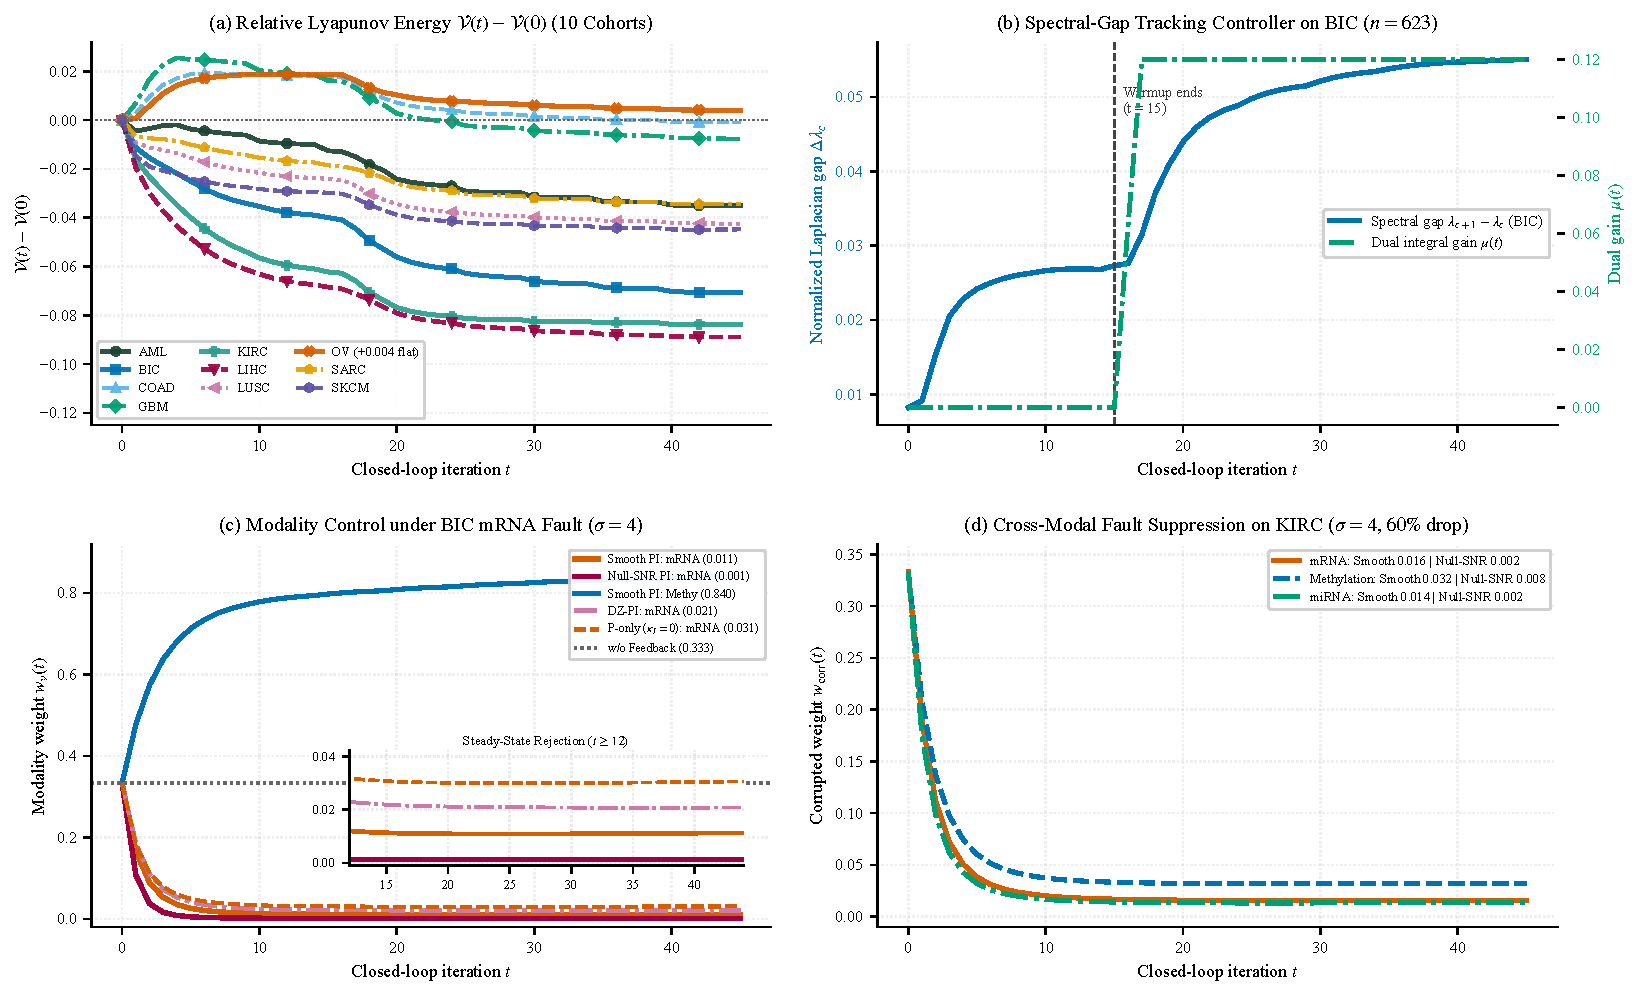
\includegraphics[width=0.89\textwidth]{figures/p2_fig2_dynamics.pdf}
    \caption{Closed-loop dynamical diagnostics. (a) Relative Lyapunov trajectory $\mathcal{V}(t)-\mathcal{V}(0)$ across 10 TCGA cohorts (non-stratified OV remains flat as an unsupervised structure monitor). (b) BIC spectral-gap tracking upon dual gain $\mu(t)$ warmup release at $t=15$. (c) BIC mRNA fault step response ($\sigma=4$): Null-SNR ($0.001$) and Smooth PI ($0.011$) remove P-only steady-state offset ($0.031$) and open-loop uniform leakage ($0.333$). (d) KIRC cross-channel attenuation.}
    \label{fig:p2_dynamics}
\end{figure*}

\subsection{Linear-Time Bipartite Landmark Controller}
For large $n \gg 10^4$, \textbf{CL-VSSC-Anchor} selects $m \ll n$ landmarks using MiniBatch k-means on initial $Z(0)$ and builds row-stochastic cell--anchor affinities $B^{(v)} \in \mathbb{R}^{n \times m}$ with $k_a$ nearest anchors per cell. Consensus bipartite fusion $B_{\mathrm{w}}(t)$ combines views globally ($\sum_v w_v B^{(v)}$) or per anchor using column weights $W_{\mathrm{loc}}(t) \in \mathbb{R}^{m \times V}$ under double-centered local feedback.

\begin{proposition}[Linear-Time Exact Equivalence from the Anchor Gram Matrix]
Let $D_r = \operatorname{diag}(B\mathbf{1}_m)$, $D_c = \operatorname{diag}(B^\top \mathbf{1}_n)$, and $\tilde{B} = D_r^{-1/2} B D_c^{-1/2}$. The bottom-$c$ eigenvectors $F \in \mathbb{R}^{n \times c}$ of the implicit two-hop Laplacian $L_{\mathrm{bip}} = I_n - \tilde{B}\tilde{B}^\top$ coincide identically with the top-$c$ left singular vectors of $\tilde{B}$, computed in $\mathcal{O}(n m^2 + m^3)$ time from the $m \times m$ Gram eigendecomposition $\tilde{B}^\top \tilde{B} = U_{\mathcal{A}} \Sigma^2 U_{\mathcal{A}}^\top$ as $F = \tilde{B} U_{\mathcal{A},:,1:c} \Sigma_{1:c}^{-1}$ with eigenvalues $\lambda_j = 1 - \sigma_j^2$.
\end{proposition}

Applying cell--anchor distance pruning directly against dual anchor coordinates gives $\mathcal{O}(T(nm^2 + \sum_v n d_v r))$ total complexity and linear $\mathcal{O}(Vnm + \sum_v nd_v)$ memory, replacing the $\mathcal{O}(n^3)$ time and $\mathcal{O}(n^2)$ memory bottlenecks of dense consensus graph learners \cite{nie2016clr,zhan2019mcgc}. Per-view consensus cuts likewise evaluate as $c - \|\tilde{B}^{(v)\top} F\|_F^2$ without forming $n \times n$ matrices.

To model locally heterogeneous assay quality across cell populations without introducing global integral bias across orthogonal views, \textbf{Double-Centered Anchor-Local PI} computes normalized consensus anchor barycenters $\hat{F}_{\mathrm{anc}}$, local cut mismatches $l_{jv}$, and anchor-and-view double-centered deviations $\tilde{\delta}_{jv}^{\mathrm{loc}}$:
\begin{equation}
\begin{aligned}
\hat{F}_{\mathrm{anc}} &= \operatorname{rownorm}(D_c^{-1} B_S^\top \hat{F}), \\
l_{jv} &= \frac{\sum_i B_{ij}^{(v)} \|\hat{f}_i - \hat{f}_{\mathrm{anc},j}\|_2^2}{2\sum_i B_{ij}^{(v)} + \varepsilon}, \\
\tilde{\delta}_{jv}^{\mathrm{loc}} &= \operatorname{clip}\!\left(l_{jv} - \bar{l}_{\cdot v} - \bar{l}_{j\cdot} + \bar{l}_{\cdot\cdot},\; -0.25,\; 0.25\right).
\end{aligned}
\label{eq:p2_local}
\end{equation}
These deviations drive anchor-wise PI errors $e_{jv}^{\mathrm{loc}} = e_v + \alpha_{\mathrm{loc}} \tilde{\delta}_{jv}^{\mathrm{loc}}$ ($\alpha_{\mathrm{loc}} = 0.25$), with global view summary $w_v = \frac{1}{m}\sum_j W_{\mathrm{loc},jv}$.

\subsection{Cut-and-SNR Sensor, Damped PI Control, and ISS Bounds}
Using effective degree-of-freedom factor $\phi_v \in [0.25, 1]$ to normalize relative reconstruction error $\tilde{r}_v(t)$, the feedback sensor scores each view as
\begin{equation}
e_v(t) = \frac{1}{c_{\mathrm{norm},v}}\,\frac{1}{c} J_{\mathrm{spec},v} + \frac{\gamma_{\mathrm{cons}}}{c}\operatorname{Tr}(F^\top L_v F) + \gamma_{\mathrm{rec}}\,\tilde{r}_v(t),
\label{eq:p2_sensor}
\end{equation}
where $c_{\mathrm{norm},v} = 1$ in baseline Smooth PI and $c_{\mathrm{norm},v} = \max(0.05, c_v^{\mathrm{null}})$ in \textbf{Null-SNR PI}, estimated from column-permuted modality graphs to remove feature-dimension bias. Setting $d_v = e_v$ defines \textbf{Smooth PI} ($\delta_{\mathrm{dz}} = 0$), whereas $d_v = \max(0, e_v - \min_u e_u - \delta_{\mathrm{dz}})$ defines dead-zone gating (\textbf{DZ-PI}). A leaky fault integrator ($\beta_I = 0.40$) drives simplex mirror descent \cite{beck2003mirror}:
\begin{equation}
\begin{aligned}
I_v(t+1) &= (1 - \beta_I) I_v(t) + \beta_I d_v(t), \\
w_v(t+1) &= \frac{w_v(t)^{1-\eta_w}\exp\!\left(-\frac{\eta_w}{\tau}\bar{u}_v(t+1)\right)}{\sum_{j=1}^V w_j(t)^{1-\eta_w}\exp\!\left(-\frac{\eta_w}{\tau}\bar{u}_j(t+1)\right)},
\end{aligned}
\label{eq:p2_w_upd}
\end{equation}
with zero-centered control signal $\bar{u}_v$ formed from $u_v = d_v + \kappa_I I_v$. Because $\beta_I \in (0, 1]$ and $I(0) = \mathbf{0}$, the leaky integrator acts as an anti-windup first-order filter satisfying the bounded-input bounded-output (BIBO) bound $0 \le I_v(t) \le \max_{0 \le s < t} d_v(s)$; this keeps early Stiefel alignment transients ($t < t_{\mathrm{warm}}$) from saturating the simplex while converging to $I_v^* = d_v^*$ at equilibrium. Internally, the controller monitors a surrogate closed-loop energy functional combining reconstruction residual, Ky Fan trace violation, simplex entropy, and consensus cut:
\begin{equation}
\begin{aligned}
\mathcal{V}(t) &= \sum_{v=1}^V w_v \tilde{r}_v + \mu_{\max} J_{\mathrm{spec}} \\
&\quad + \tau \sum_{v=1}^V w_v \log w_v + \frac{\alpha}{c} \sum_{v=1}^V w_v e_{\mathrm{cut},v}.
\end{aligned}
\label{eq:p2_lyap}
\end{equation}

\begin{proposition}[Simplex Optimality and Exponential PI Attenuation]
For $\eta_w \in (0, 1]$ and $\tau > 0$ initialized at $w(0) = \frac{1}{V}\mathbf{1}$, update \eqref{eq:p2_w_upd} minimizes a strictly convex KL-regularized simplex objective, keeping $w(t) \in \mathrm{int}(\Delta^V)$ and bounded $(e_v, \mathcal{V})$. At Smooth PI equilibrium ($\delta_{\mathrm{dz}} = 0$), any degraded view $b$ exceeding a clean view $g$ by $\Delta e = e_b^* - e_g^* > 0$ obeys $w_b^*/w_g^* = \exp(-(1+\kappa_I)\Delta e / \tau)$, whereas $\delta_{\mathrm{dz}} > 0$ weakens attenuation to $\exp(-(1+\kappa_I)\max(0,\Delta e - \delta_{\mathrm{dz}})/\tau)$ and stalls feedback when $\Delta e \le \delta_{\mathrm{dz}}$.
\end{proposition}

\begin{proposition}[Local ISS and Davis--Kahan Bound]
Let $L^* = L(S^*)$ denote the oracle clean consensus Laplacian with eigengap $\Delta\lambda_c^* > 0$ and subspace $F^*$. Assume coupling gains $(\gamma_{\mathrm{cons}}, \lambda_Z)$ keep trajectories inside the decoupled basin where corrupted views $b \in \mathcal{B}$ keep $\Delta e_b > 0$ with bounded discrepancy $\Delta_L$ and pruning perturbation $\bar{\delta}_\mu$. Within this basin, $\|L(S(t)) - L^*\|_F$ contracts at rate $(1-\eta_S)^t$ toward $\Delta_\infty \le \sum_{b \in \mathcal{B}} w_b^* \Delta_L + \bar{\delta}_\mu$, ensuring local ISS \cite{sontag2008iss}. For any gap $\Delta_\infty < \Delta\lambda_c^*$, Davis--Kahan's theorem \cite{davis1970rotation} gives
\begin{equation}
\begin{aligned}
\|\sin\Theta(F^*, F_\infty)\|_F &\le \frac{2\sqrt{c}}{\Delta\lambda_c^* - \Delta_\infty} \\
&\quad \times \left(\Delta_L \sum_{b \in \mathcal{B}} e^{-\frac{1+\kappa_I}{\tau}\Delta e_b} + \bar{\delta}_\mu\right).
\end{aligned}
\label{eq:p2_dk}
\end{equation}
\end{proposition}

Equations~\eqref{eq:p2_w_upd} and~\eqref{eq:p2_dk} also clarify the loop-gain trade-off mapped later in Fig.~\ref{fig:p2_phase_200k}(a): raising the effective PI gain $K_{\mathrm{eff}} = K_p(1 + \kappa_I) = \frac{\eta_w}{\tau}(1+\kappa_I)$ tightens the numerator of \eqref{eq:p2_dk}, whereas excessive $K_p$ or $\kappa_I$ violates the discrete small-gain condition on $S(t)$ and induces limit-cycle ringing or premature single-view lock-in. All proofs and full symbol/complexity details appear in Appendix~\ref{app:proofs} and Supplementary Material (Sections~S1--S2). Algorithm~\ref{alg:cl_vssc} summarizes unified execution under fixed global parameters ($r=24$, $r_v=6$, $\lambda_Z=2.0$, $\eta_Z=\eta_S=0.35$, $\gamma_{\mathrm{rec}}=0.30$, $\gamma_{\mathrm{cons}}=0.08$, $\eta_w=0.30$, $\beta_I=0.40$, $\kappa_I=0.35$, $\tau=0.20$, $\eta_\mu=0.05$, $\mu_{\max}=0.12$, $\epsilon_{\mathrm{spec}}=0.02$).

\begin{algorithm}[t]
\caption{CL-VSSC / CL-VSSC-Anchor Closed-Loop Control}
\label{alg:cl_vssc}
\begin{algorithmic}[1]
\REQUIRE Views $\{X^{(v)}\}_{v=1}^V$, cluster count $c$, mode (\textsc{Dense} or \textsc{Anchor} with $m$ landmarks).
\ENSURE Partitions $\hat{y}$, weights ($w$ / $W_{\mathrm{loc}}$), trajectories $(\mathcal{V}, w, \Delta\lambda_c, \mu)$.
\STATE Initialize Stiefel state $Z$, specific factors $U^{(v)}$, view graphs ($A^{(v)}$ or $B^{(v)}$), $w \leftarrow \frac{1}{V}\mathbf{1}$, $I \leftarrow \mathbf{0}$, $\mu \leftarrow 0$, and $F(0)$.
\FOR{$t = 0$ to $T-1$}
    \STATE Update shared $Z(t+1)$ with \eqref{eq:p2_plant} and nuisance factors $U^{(v)} \perp Z$.
    \STATE Periodically refresh $A^{(v)}$ (\textsc{Dense}) or $B^{(v)}$ (\textsc{Anchor}).
    \STATE Update fused actuator and dual gain $\mu(t+1)$ with \eqref{eq:p2_dual}; extract $F(t+1)$ (Prop.~1 in \textsc{Anchor}).
    \STATE Evaluate sensor $e_v(t)$ from \eqref{eq:p2_sensor} (plus \eqref{eq:p2_local} for local PI); update weights \eqref{eq:p2_w_upd} and log $\mathcal{V}(t+1)$ with \eqref{eq:p2_lyap}.
\ENDFOR
\STATE Assign clusters $\hat{y}$ using $k$-means on row-normalized $F(T)$.
\end{algorithmic}
\end{algorithm}

\section{Experimental Protocol}

\subsection{TCGA Multi-Modality Fault Stress and Sensitivity Grids}
Clean dynamical diagnostics and 5{,}000-permutation survival evaluations (\texttt{lifelines} \cite{davidsonpilon2019lifelines}) spanned all $10$ TCGA cohorts ($N=3{,}113$, $1{,}235$ events; mRNA, DNA methylation, miRNA \cite{rappoport2018multi}) in \texttt{PyTorch 2.14} \cite{paszke2019pytorch}. Three-modality stress testing was conducted across BIC, KIRC, LIHC, and GBM by injecting Gaussian noise plus random dropout across five severity levels from $\sigma=0.0$ ($0\%$ drop) to $\sigma=4.0$ ($60\%$ drop) over $3$ seeds ($3$ seeds per cohort--modality--severity cell across $10$ evaluated configurations). Statistical comparisons across paired runs used one-sided paired Wilcoxon signed-rank tests with Benjamini--Hochberg false discovery rate (BH-FDR) $q$-values. Sensitivity grids swept $\kappa_I \times \tau$ ($25$ pairs), $\mu_{\max} \in [0.0, 0.24]$, and anchor count $m \in [128, 768]$ on BIC, KIRC, and \texttt{BMMC-10k}. To delineate classical gain-margin regimes on A100-80GB, we further mapped $536$ points over $K_p = \eta_w/\tau \in [0.25, 40.0]$ and $\kappa_I = K_i / K_p \in [0.0, 10.0]$ ($\eta_w = 0.30$) across $\delta_{\mathrm{dz}} \in \{0.00, 0.05, 0.14, 0.25\}$ on clean and $\sigma=4.0$ mRNA-faulted BIC and KIRC ($11\times 11$ at $\delta_{\mathrm{dz}}=0$, $7\times 7$ common subset per nonzero $\delta_{\mathrm{dz}}$).

\subsection{CITE-seq Atlas, 300k Scaling, and 200k Self-Healing}
External ground-truth clustering accuracy (ARI, NMI, ACC) without survival proxies was measured on the NeurIPS \texttt{GSE194122} CITE-seq atlas ($90{,}261$ human bone marrow cells, $13{,}953$ genes, $134$ surface ADTs, $45$ annotated cell types across $4$ sites \cite{luecken2021sandbox}). Using top-$2{,}000$ HVG log-normalized RNA and CLR-normalized ADT counts on \texttt{BMMC-\allowbreak Site1} ($32{,}004$), \texttt{BMMC-\allowbreak Site2} ($25{,}161$), \texttt{BMMC-\allowbreak 10k}, and \texttt{BMMC-\allowbreak 30k} ($3$ seeds), we tested clean integration, \texttt{BMMC-\allowbreak 10k} scRNA/ADT fault stress ($\sigma \in \{0, 1.5, 3.0\}$), and scaling curves from $1{,}000$ to $90{,}261$ cells (A100 for global modes; L4 for Anchor-Local PI). To stress-test ultra-large-scale convergence on A100-80GB, we extended scaling from $10{,}000\text{--}90{,}261$ real \texttt{GSE194122} cells up to $150{,}000\text{--}300{,}000$ cells by stratified sampling with $\mathcal{N}(0, 0.05\sigma_j)$ manifold jitter (\texttt{GSE194122-\allowbreak Expanded}, using \texttt{MiniBatchKMeans} beyond $100{,}000$ cells), and measured static ($t=0$) and mid-stream ($t=10$) Protein-ADT step-fault self-healing ($\sigma=3.0$, $50\%$ dropout) at $N=200{,}000$.

\section{Experimental Results}

\subsection{Closed-Loop Dynamics and Controller Ablations}
\begin{table*}[t]
\centering
\caption{Three-Modality Sensor-Fault Stress Summary across BIC, KIRC, LIHC, and GBM (4 Cohorts $\times$ 3 Seeds = 12 Runs per Setting; One-Sided Paired Wilcoxon BH-FDR $q$ Across $n=36$ $\sigma=4.0$ Runs, with $q = 1.46{\times}10^{-11}$ Fault-Weight Suppression vs.\ Every Weighted Baseline)}
\label{tab:p2_fault}
\scriptsize
\renewcommand{\arraystretch}{1.14}
\setlength{\tabcolsep}{2.2pt}
\begin{tabular}{llcccccccccc}
\toprule
Fault Scenario & Metric & \shortstack{CL-\\VSSC} & \shortstack{Null-\\SNR} & \shortstack{DZ-\\PI} & \shortstack{w/o\\FB} & SNF & NEMO & MCGC & \shortstack{Seurat\\WNN} & \shortstack{Att.\\MOAE} & \shortstack{Sub.\\GAN} \\
\midrule
mRNA ($\sigma{=}4.0$) & ARI retention & 0.443 & 0.643 & 0.416 & 0.489 & 0.462 & 0.498 & 0.391 & 0.460 & 0.639 & 0.185 \\
 & $-\log_{10}p_{\mathrm{asymp}}$ & 2.178 & 2.040 & 1.821 & 2.104 & 2.265 & 2.241 & 2.628 & 2.338 & 1.399 & 1.830 \\
 & Fault weight & 0.011 & 0.001 & 0.022 & 0.333 & --- & --- & 0.172 & 0.258 & 0.314 & --- \\
\midrule
Methylation ($\sigma{=}4.0$) & ARI retention & 0.214 & 0.170 & 0.271 & 0.295 & 0.361 & 0.310 & 0.361 & 0.294 & 0.439 & 0.158 \\
 & $-\log_{10}p_{\mathrm{asymp}}$ & 1.865 & 1.891 & 1.560 & 1.825 & 1.390 & 1.661 & 2.052 & 1.965 & 2.206 & 1.238 \\
 & Fault weight & 0.017 & 0.003 & 0.031 & 0.333 & --- & --- & 0.189 & 0.276 & 0.308 & --- \\
\midrule
miRNA ($\sigma{=}4.0$) & ARI retention & 0.796 & 0.949 & 0.715 & 0.576 & 0.615 & 0.579 & 0.491 & 0.607 & 0.414 & 0.207 \\
 & $-\log_{10}p_{\mathrm{asymp}}$ & 1.911 & 2.131 & 1.929 & 2.054 & 1.779 & 2.200 & 2.881 & 2.397 & 1.833 & 2.109 \\
 & Fault weight & 0.009 & 0.001 & 0.018 & 0.333 & --- & --- & 0.209 & 0.259 & 0.334 & --- \\
\midrule
All assays ($\sigma{=}2.0$, 45\%) & ARI retention & 0.482 & \textbf{0.593} & 0.475 & 0.503 & 0.500 & 0.479 & 0.430 & 0.477 & 0.513 & 0.188 \\
 & $-\log_{10}p_{\mathrm{asymp}}$ & 1.978 & 1.999 & 1.789 & 1.930 & 1.887 & 2.134 & 2.526 & 2.268 & 1.740 & 1.652 \\
 & Fault weight & \textbf{0.018} & \textbf{0.003} & 0.035 & 0.333 & --- & --- & 0.200 & 0.266 & 0.318 & --- \\
\midrule
All assays ($\sigma{=}4.0$, 60\%) & ARI retention & 0.484 & \textbf{0.587} & 0.467 & 0.453 & 0.479 & 0.463 & 0.415 & 0.454 & 0.497 & 0.184 \\
 & $-\log_{10}p_{\mathrm{asymp}}$ & 1.985 & 2.021 & 1.770 & 1.994 & 1.811 & 2.034 & 2.520 & 2.233 & 1.813 & 1.726 \\
 & Fault weight & \textbf{0.012} & \textbf{0.002} & 0.024 & 0.333 & --- & --- & 0.190 & 0.264 & 0.319 & --- \\
 & BH-FDR $q$ (vs.\ Null) & 0.010 & --- & 0.005 & 0.010 & 0.020 & 0.010 & 0.005 & 0.010 & 0.177 & $2.2{\times}10^{-6}$ \\
\bottomrule
\end{tabular}
\end{table*}


\begin{figure*}[t]
    \centering
    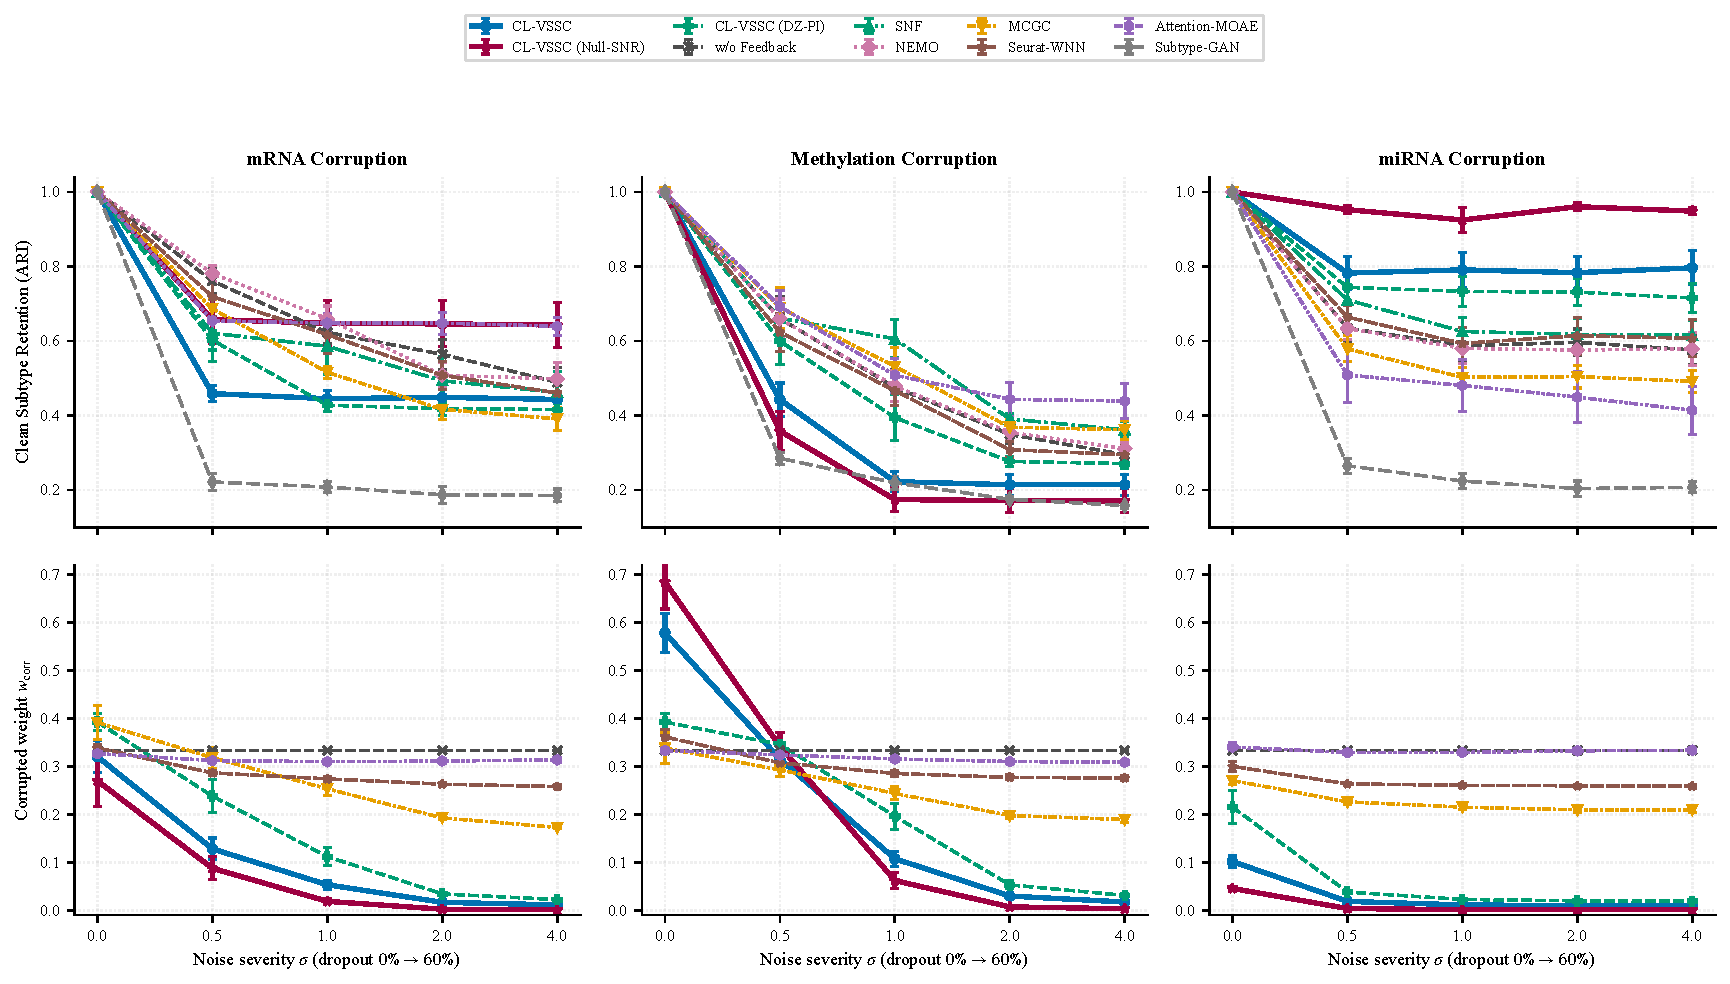
\includegraphics[width=0.84\textwidth]{figures/p2_fig3_fault_tolerance.pdf}
    \caption{Three-modality fault-tolerance profiles ($\pm 1$ SE over 12 runs/point). Top: clean subtype ARI retention across noise severity $\sigma \in [0, 4]$. Bottom: converged faulty-modality weight showing Smooth PI ($0.009\text{--}0.017$) and Null-SNR PI ($0.001\text{--}0.003$) crushing degraded sensors while open-loop baselines retain $0.172\text{--}0.334$.}
    \label{fig:p2_fault}
\end{figure*}

Table~\ref{tab:p2_ablation} and Fig.~\ref{fig:p2_dynamics} isolate each control loop. Consistent with Proposition~2, \textbf{Smooth PI} ($\delta_{\mathrm{dz}} = 0$) achieves stronger clean stratification ($5/10$ cohorts; median $1.248$; $k$-sweep $23/40$; Silhouette $0.509$) and tighter severe-fault attenuation ($w_{\mathrm{corr}} = 0.012$) than rigid \textbf{DZ-PI} ($4/10$; median $0.845$; $w_{\mathrm{corr}} = 0.024$). Removing integral memory (\textbf{P-only}, $\kappa_I=0$) leaves nearly $3\times$ higher faulty mRNA weight on BIC ($0.031$ vs.\ $0.011$; Fig.~\ref{fig:p2_dynamics}(c)), whereas disabling feedback fixes leakage at $0.333$. Internally, the surrogate closed-loop energy $\mathcal{V}(t)$ achieves net descent ($\mathcal{V}(T) < \mathcal{V}(0)$) following early warmup transients in $9/10$ clean TCGA cohorts (diagnostic non-stratified OV remains near flat at $+0.004$; Fig.~\ref{fig:p2_dynamics}(a)). Releasing $\mu(t)$ at $t=15$ widens the BIC eigengap $6.70\times$ ($0.0082 \rightarrow 0.0550$; Fig.~\ref{fig:p2_dynamics}(b)).

Enabling \textbf{Null-SNR PI} highlights a sensor gain trade-off. Normalizing cuts against shuffled null baselines raises clean Silhouette ($0.509 \rightarrow 0.516$) and sharpens GBM ($3.097 \rightarrow 3.699$) and KIRC ($2.377 \rightarrow 2.523$). However, it attenuates lower-dimensional miRNA weights ($0.035\text{--}0.099$), trimming clean TCGA significance to $3/10$ (median $0.882$) in exchange for stronger heavy-fault rejection below.

\subsection{Three-Modality Sensor-Fault Tolerance}
\begin{table*}[t]
\centering
\caption{Single-Cell CITE-seq Benchmark (GSE194122 BMMC, 39--45 Cell Types), Protein ADT Fault ($\sigma=3.0$), and 90{,}261-Cell Scaling ($^\dagger$L4 GPU)}
\label{tab:p2_singlecell}
\scriptsize
\renewcommand{\arraystretch}{1.14}
\setlength{\tabcolsep}{2.0pt}
\begin{tabular}{lccccccc}
\toprule
Method & \shortstack{BMMC-Site1\\($32{,}004$, NMI/ACC)} & \shortstack{BMMC-Site2\\($25{,}161$, NMI/ACC)} & \shortstack{BMMC-10k\\(NMI/ACC)} & \shortstack{BMMC-30k\\(NMI/ACC)} & \shortstack{BMMC-10k ADT Fault\\($\sigma=3$, ARI/ACC)} & \shortstack{ADT Fault\\$w_{\mathrm{ADT}}$} & \shortstack{90{,}261 Cells\\Time (s) / MB} \\
\midrule
CL-VSSC-Anchor & 0.586 / 0.325 & 0.668 / 0.394 & 0.588 / 0.308 & 0.585 / 0.312 & \textbf{0.169} / \textbf{0.282} & 0.317 & 16.57 / 5,295 \\
Anchor (Local PI) & 0.585 / 0.319 & 0.667 / 0.401 & 0.592 / 0.312 & 0.587 / 0.316 & 0.156 / 0.276 & 0.324 & 21.71$^\dagger$ / 5,434 \\
Anchor (Local+Null) & 0.587 / 0.324 & 0.668 / 0.394 & 0.593 / 0.316 & 0.586 / 0.319 & 0.157 / 0.279 & 0.299 & 22.08$^\dagger$ / 5,434 \\
Anchor (Null-SNR) & 0.589 / 0.328 & 0.668 / 0.397 & 0.591 / 0.313 & 0.583 / 0.313 & 0.166 / 0.279 & 0.294 & --- \\
Anchor (DZ-PI) & 0.596 / 0.324 & 0.673 / 0.397 & 0.599 / 0.315 & 0.597 / 0.319 & 0.123 / 0.227 & 0.500 & --- \\
Anchor (w/o FB) & 0.597 / 0.326 & 0.674 / 0.402 & 0.614 / 0.338 & 0.609 / 0.334 & 0.123 / 0.227 & 0.500 & --- \\
LMVSC & 0.603 / 0.336 & 0.666 / 0.382 & 0.600 / 0.325 & 0.603 / 0.331 & 0.162 / 0.274 & --- & 7.06 / 2,141 \\
Seurat-WNN & 0.609 / 0.340 & 0.680 / 0.398 & 0.618 / 0.334 & 0.614 / 0.340 & 0.155 / 0.270 & 0.494 & --- \\
Attention-MOAE & 0.616 / 0.341 & 0.683 / 0.404 & 0.633 / 0.347 & 0.624 / 0.361 & 0.051 / 0.108 & 0.866 & --- \\
Subtype-GAN & 0.583 / 0.331 & 0.650 / 0.438 & 0.548 / 0.313 & 0.568 / 0.341 & 0.087 / 0.122 & --- & 36.40 / 805 \\
\bottomrule
\end{tabular}
\end{table*}


\begin{figure*}[t]
    \centering
    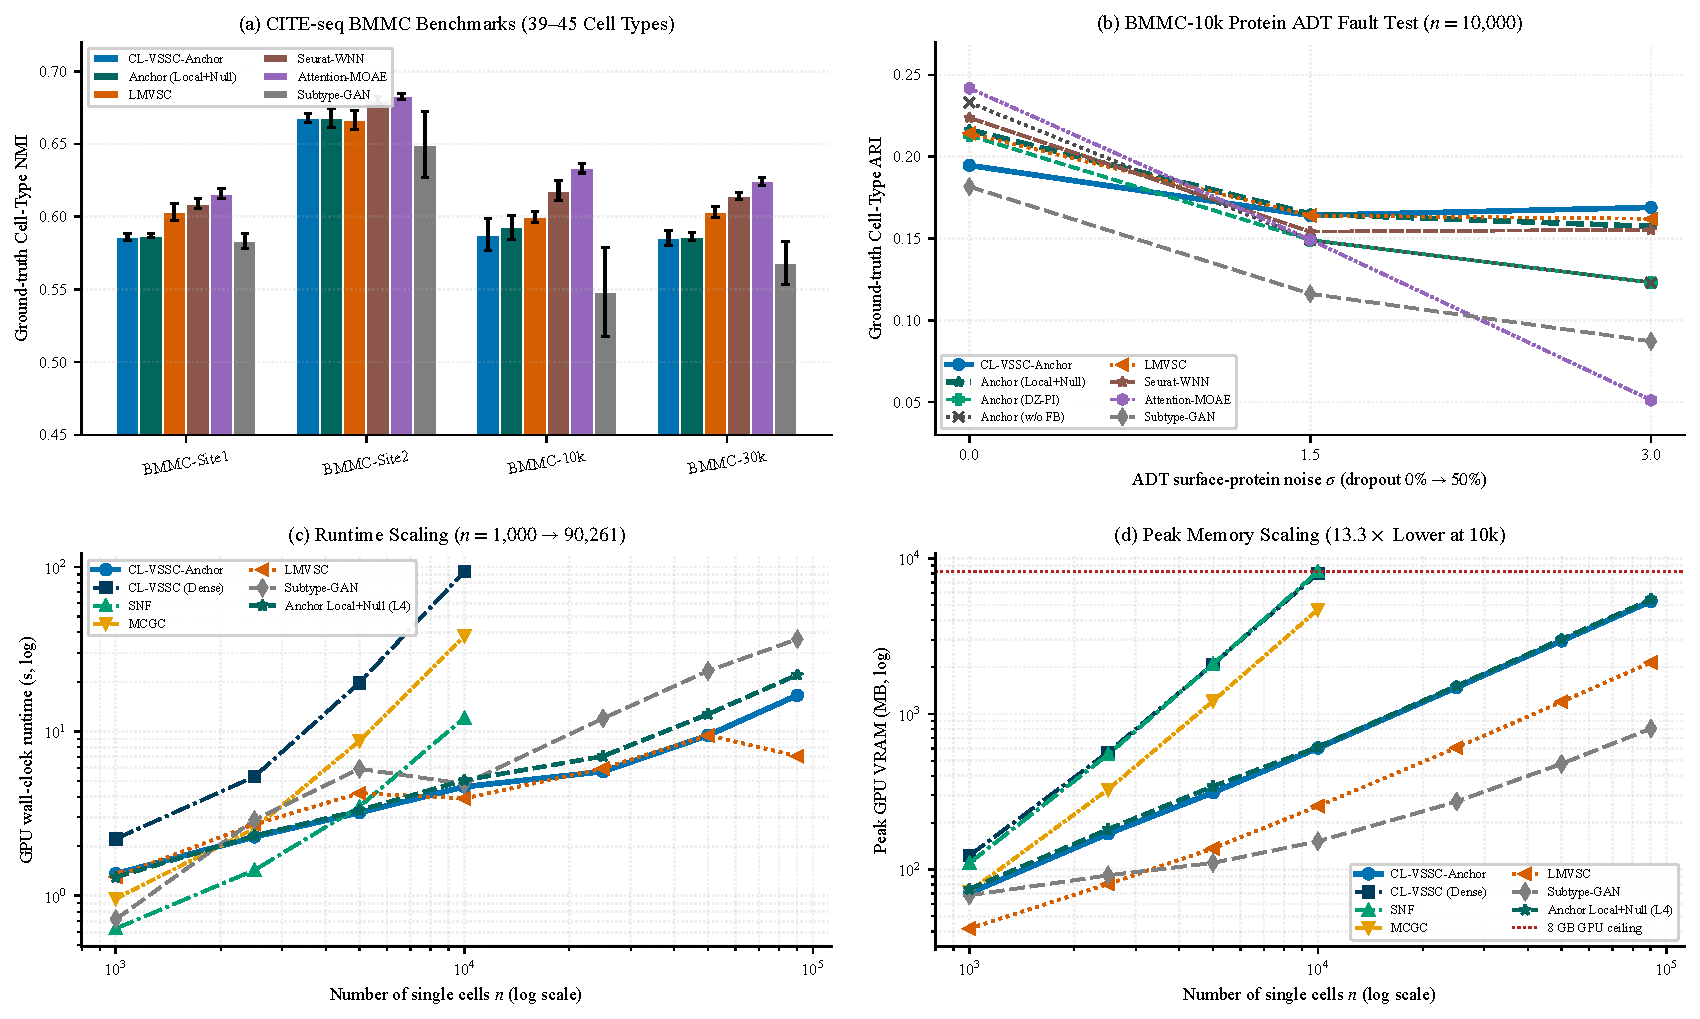
\includegraphics[width=0.80\textwidth]{figures/p2_fig4_singlecell_scale.pdf}
    \caption{NeurIPS GSE194122 single-cell CITE-seq validation ($90{,}261$ BMMCs, $39\text{--}45$ cell types). (a) Clean multi-site NMI. (b) \texttt{BMMC-10k} ADT fault test ($\sigma \in [0,3]$): CL-VSSC-Anchor leads all competitors ($\mathrm{ARI}=0.169$) while Attention-MOAE collapses ($0.051$). (c)--(d) Log--log GPU runtime and peak VRAM scaling ($1{,}000 \rightarrow 90{,}261$ cells).}
    \label{fig:p2_singlecell}
\end{figure*}

Table~\ref{tab:p2_fault} and Fig.~\ref{fig:p2_fault} evaluate severe cross-assay corruption. At $\sigma=4.0$ ($60\%$ drop), Smooth PI attenuates faulty modalities to $0.012$ mean weight, which is $15.8\times$ tighter than MCGC ($0.190$), $22.0\times$ tighter than \texttt{Seurat-\allowbreak WNN} ($0.264$), and $26.6\times$ tighter than \texttt{Attention-\allowbreak MOAE} ($0.319$). Across all $36$ paired $\sigma=4.0$ runs, both Smooth PI and Null-SNR PI suppress faulty weights below every weighted competitor ($36/36$ wins, paired Wilcoxon BH-FDR $q = 1.46\times 10^{-11}$). Layering \textbf{Null-SNR PI} cuts mean faulty weight nearly $7\times$ further to $\mathbf{0.002}$ ($0.001$ mRNA, $0.003$ Methylation, $0.001$ miRNA) and raises overall clean-label retention ARI by $+0.103$ ($0.484 \rightarrow \mathbf{0.587}$), leading all $10$ configurations at both $\sigma=2.0$ ($0.593$ ARI) and $\sigma=4.0$ ($0.587$ ARI; statistically higher than $8/9$ methods at BH-FDR $q \le 0.0196$, and $q \le 3.47\times 10^{-3}$ across combined severe faults $\sigma \in \{2.0, 4.0\}$, $n=72$). On secondary-assay corruption (mRNA and miRNA, $n=24$ at $\sigma=4.0$) where primary methylation structure stays observable, Null-SNR PI attains $0.796$ mean ARI ($0.949$ miRNA, $0.643$ mRNA) vs.\ $0.526$ for \texttt{Attention-\allowbreak MOAE} and $0.441$ for MCGC, outperforming all $9/9$ competitors ($q \le 6.19\times 10^{-4}$). Methylation retention is lower ($0.170$ vs.\ $0.214$) because corrupting DNA methylation directly degrades the strongest primary assay in GBM and KIRC even when $w_{\mathrm{methy}} = 0.003$.

\subsection{90,261-Cell CITE-seq Benchmark and Linear Scaling}
\begin{figure*}[t]
    \centering
    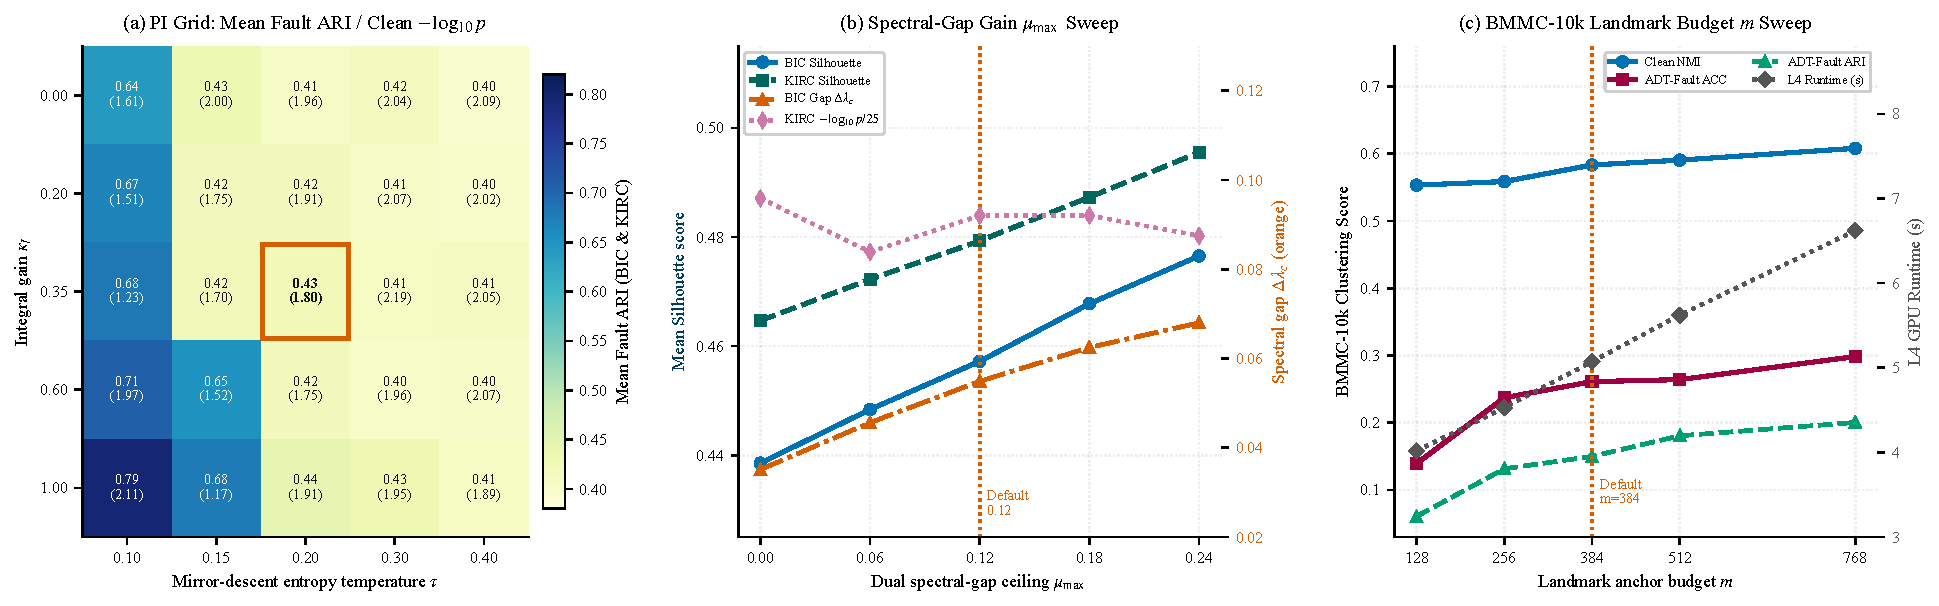
\includegraphics[width=0.78\textwidth]{figures/p2_fig5_sensitivity.pdf}
    \caption{Control-parameter sensitivity sweeps. (a) $(\kappa_I \times \tau)$ grid averaged over BIC and KIRC showing Fault ARI and clean $-\log_{10}p_{\mathrm{perm}}$ (default boxed in orange). (b) Monotonic Silhouette and spectral-gap expansion across $\mu_{\max} \in [0, 0.24]$. (c) Monotonic clustering and ADT-fault gains across landmark count $m \in [128, 768]$ within sub-7s L4 runtime.}
    \label{fig:p2_sensitivity}
\end{figure*}

Table~\ref{tab:p2_singlecell} and Fig.~\ref{fig:p2_singlecell} validate CL-VSSC-Anchor on $90{,}261$ real single cells. On clean multi-site CITE-seq (Fig.~\ref{fig:p2_singlecell}(a)), \textbf{Double-Centered Anchor-Local PI} ($\alpha_{\mathrm{loc}}=0.25$) and \textbf{Local+Null} avoid global integral drift across complementary RNA and ADT views, improving clean ARI over global CL-VSSC-Anchor in $9/12$ paired runs ($p = 0.032$, one-sided Wilcoxon) on high-heterogeneity marrow cohorts (\texttt{BMMC-\allowbreak 10k}: ARI $0.201 \rightarrow 0.218$, NMI $0.588 \rightarrow 0.593$, ACC $0.308 \rightarrow 0.316$; \texttt{BMMC-\allowbreak 30k}: ARI $0.212 \rightarrow 0.222$, ACC $0.312 \rightarrow 0.319$; \texttt{BMMC-\allowbreak Site2}: ACC $0.394 \rightarrow 0.401$). When Protein ADT undergoes $\sigma=3.0$ noise and $50\%$ dropout on \texttt{BMMC-\allowbreak 10k} (Fig.~\ref{fig:p2_singlecell}(b)), \texttt{Attention-\allowbreak MOAE} stays locked to ADT ($w_{\mathrm{ADT}}=0.866$) and drops $-78.9\%$ in ARI ($0.242 \rightarrow 0.051$), \texttt{Subtype-\allowbreak GAN} falls to $0.087$, and DZ-PI stalls at $0.500$ ($0.123$ ARI). CL-VSSC-Anchor downweights corrupted ADT to $0.317$ and leads all baselines ($\mathrm{ARI}=0.169$, $\mathrm{ACC}=0.282$; winning $6/6$ paired runs across $\sigma \in \{1.5, 3.0\}$, $p = 0.0156$, against \texttt{Attention-\allowbreak MOAE}, \texttt{Subtype-\allowbreak GAN}, DZ-PI, and \texttt{w/o FB}), while Null-SNR ($0.294$) and Local+Null ($0.299$) lower ADT leakage further. Under reverse $\sigma=3.0$ \texttt{scRNA} corruption, CL-VSSC-Anchor ($w_{\mathrm{RNA}}=0.069$) and Null-SNR ($0.060$) likewise isolate RNA noise ($\mathrm{ARI}=0.208\text{--}0.213$), whereas \texttt{Attention-\allowbreak MOAE} assigns static high ADT weight ($0.891$) in both directions (Supplementary Material, Sections~S3--S4).

Across $1{,}000 \rightarrow 90{,}261$ cells (Fig.~\ref{fig:p2_singlecell}(c)--(d)), CL-VSSC-Anchor reduces $10{,}000$-cell A100 runtime $20.3\times$ ($4.60\text{ s}$ vs.\ $93.58\text{ s}$ Dense) and peak VRAM $13.3\times$ ($603\text{ MB}$ vs.\ $8{,}002\text{ MB}$). It completes all $90{,}261$ cells in $16.57\text{ s}$ at $5{,}295\text{ MB}$ on A100 ($21.71\text{--}22.08\text{ s}$ and $5{,}434\text{ MB}$ Local PI on L4, only $+2.6\%$ peak memory overhead).

\subsection{Control-Parameter Sensitivity Frontier}
Fig.~\ref{fig:p2_sensitivity} sweeps all three controller hyperparameters to test Propositions~2 and~3 empirically. Across the $5 \times 5$ $(\kappa_I \times \tau)$ grid (Fig.~\ref{fig:p2_sensitivity}(a)), raising integral gain $\kappa_I$ and lowering entropy temperature $\tau$ shrink the exponential numerator in \eqref{eq:p2_dk}: $\sigma=4.0$ mRNA fault retention climbs from $0.350 \rightarrow 0.597$ on BIC and $0.445 \rightarrow 0.990$ on KIRC as corrupted weights vanish toward $0.000$. Setting a stiff $\tau=0.10$ at $\kappa_I=0.35$ risks premature clean-view collapse ($0.719$ BIC survival), placing $(\kappa_I=0.35, \tau=0.20)$ inside the stable Pareto basin. Sweeping $\mu_{\max} \in [0, 0.24]$ (Fig.~\ref{fig:p2_sensitivity}(b)) produces monotonic Silhouette cohesion (BIC $0.4386 \rightarrow 0.4765$; KIRC $0.4647 \rightarrow 0.4955$) and BIC eigengap expansion ($0.0351 \rightarrow 0.0680$), with clean survival peaking near $\mu_{\max}=0.12$. Sweeping landmark budget $m \in [128, 768]$ on \texttt{BMMC-\allowbreak 10k} (Fig.~\ref{fig:p2_sensitivity}(c)) improves clean NMI ($0.553 \rightarrow 0.608$) and ADT-fault ARI ($0.061 \rightarrow 0.200$) within $4.02\text{--}6.62\text{ s}$ on L4.

\subsection{PI Gain Stability Phase Diagram and 200k--300k Self-Healing}
\begin{figure*}[t]
    \centering
    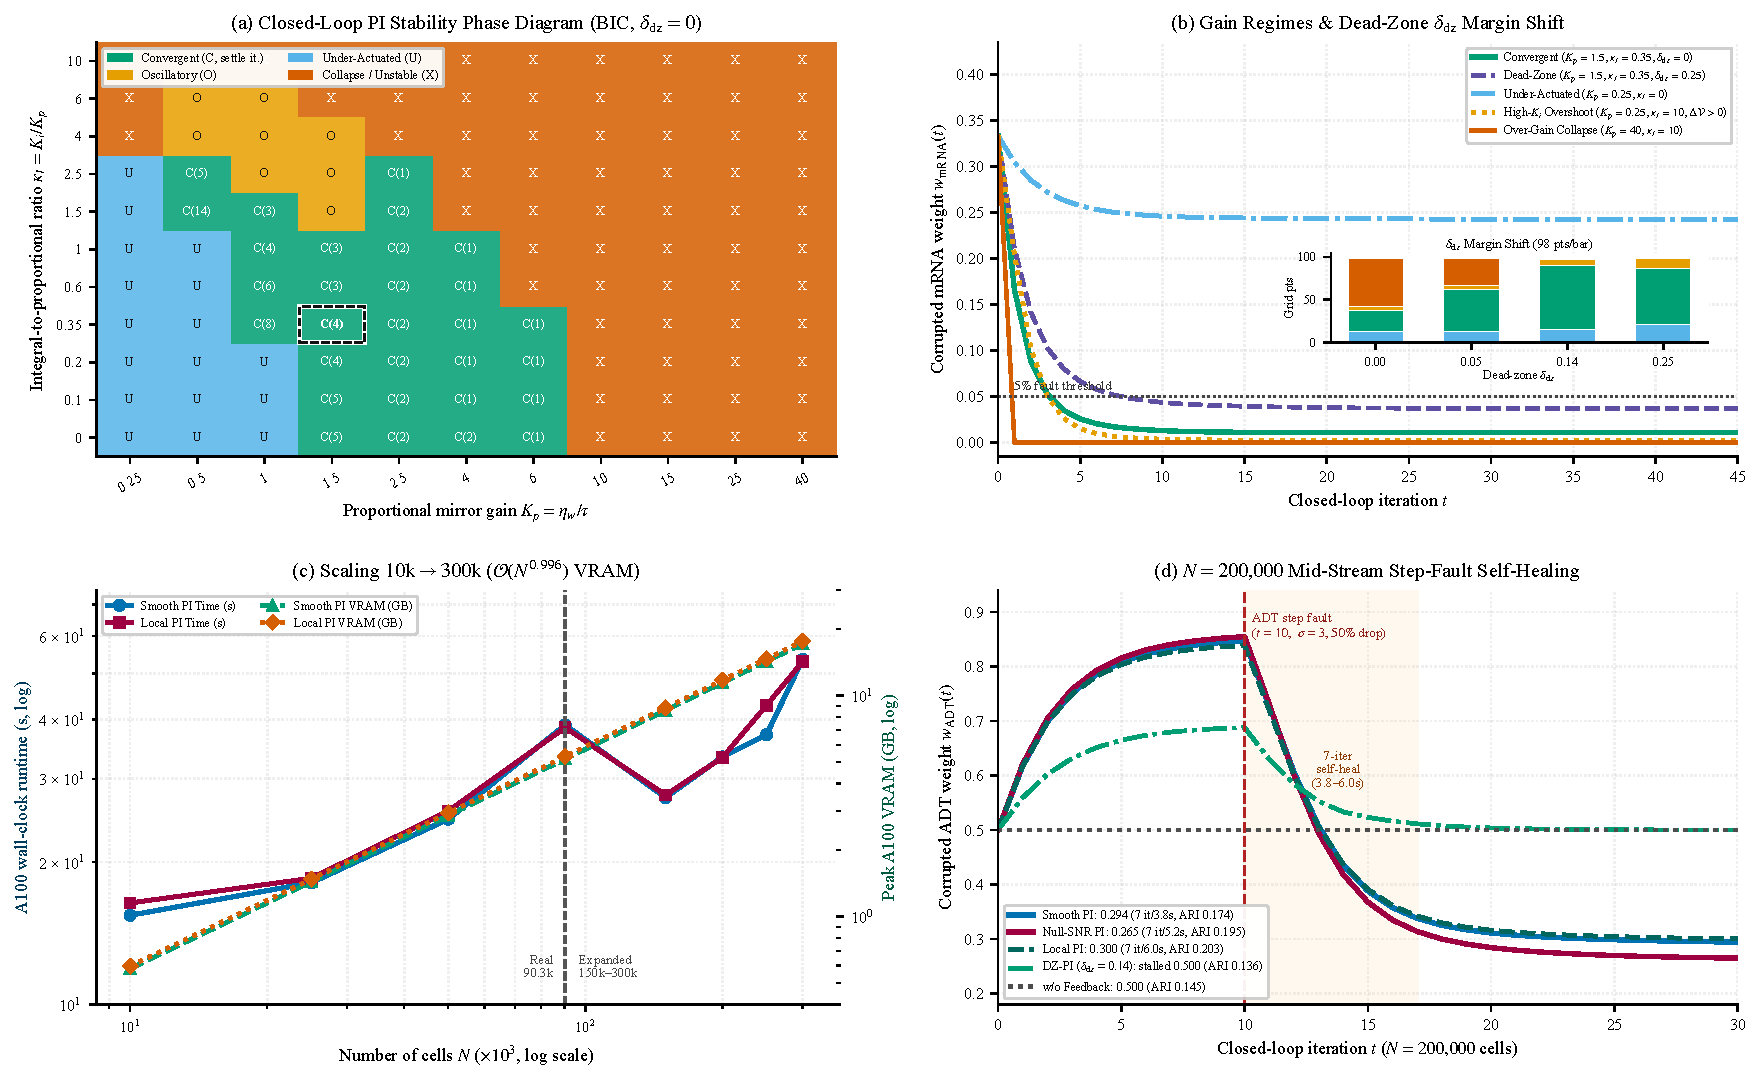
\includegraphics[width=0.83\textwidth]{figures/p2_fig6_stability_phase_200k.pdf}
    \caption{A100-80GB closed-loop stability boundaries and $200\text{k}\text{--}300\text{k}$ self-healing verification. (a) $(K_p, \kappa_I)$ stability phase diagram on BIC ($\delta_{\mathrm{dz}}=0$; default operating point boxed). (b) Representative mRNA fault trajectories and dead-zone $\delta_{\mathrm{dz}}$ margin shift (inset, $98$ BIC+KIRC points per bar). (c) Log--log scaling across $10\text{k}\text{--}300\text{k}$ cells (\texttt{GSE194122} real up to $90.3\text{k}$, \texttt{GSE194122-\allowbreak Expanded} $150\text{k}\text{--}300\text{k}$). (d) $N=200{,}000$ mid-stream ADT step-fault self-healing ($t=10$, $\sigma=3.0$, $50\%$ drop).}
    \label{fig:p2_phase_200k}
\end{figure*}

Fig.~\ref{fig:p2_phase_200k}(a)--(b) resolves the classical control stability margins predicted by Propositions~2 and~3 across $536$ $(K_p, K_i, \delta_{\mathrm{dz}})$ points. On $\delta_{\mathrm{dz}}=0$, low gains ($K_p \le 1.0$ with low $\kappa_I$) remain \emph{Under-Actuated} ($w_{\mathrm{mRNA}} > 0.05$), whereas excessive proportional ($K_p \ge 6\text{--}10$) or integral ($K_i/K_p \ge 4\text{--}10$, with $\Delta\mathcal{V} > 0$) gains enter \emph{Collapse / Unstable} single-view lock-in. Between them, an \emph{Oscillatory} transition band (non-monotone $\mathcal{V}(t)$ fraction $>0.20$) borders the well-damped \emph{Convergent} basin ($30/121$ BIC points; $15/121$ KIRC points), where the default controller ($K_p=1.5, \kappa_I=0.35$) settles in $4\text{--}5$ steps ($w_{\mathrm{mRNA}}=0.0113$ BIC, $0.0156$ KIRC). Raising $\delta_{\mathrm{dz}} \in \{0.00, 0.05, 0.14, 0.25\}$ shrinks \emph{Collapse / Unstable} counts across the common $98$-point grid ($56 \rightarrow 31 \rightarrow 1 \rightarrow 0$) at the cost of widening \emph{Under-Actuated / Stalled} zones ($13 \rightarrow 13 \rightarrow 15 \rightarrow 21$), explaining why zero dead zone preserves both gain margin and sensitivity inside the ISS basin.

Across $10{,}000 \rightarrow 300{,}000$ cells on \texttt{A100-SXM4-80GB} (Fig.~\ref{fig:p2_phase_200k}(c)), peak VRAM follows exact linear scaling ($\mathcal{O}(N^{0.9955})$, $594.8\text{ MB} \rightarrow 17{,}546.7\text{ MB}$ Smooth PI; $611.4\text{ MB} \rightarrow 18{,}037.8\text{ MB}$ Local PI) with sub-minute $300{,}000$-cell completion ($53.56\text{ s}$ Smooth PI, $52.98\text{ s}$ Local PI; empirical runtime exponent $0.3106$ aided by \texttt{MiniBatchKMeans} beyond $100{,}000$ cells) and monotonic Lyapunov descent at every scale. At $N=200{,}000$ (Fig.~\ref{fig:p2_phase_200k}(d)), injecting a mid-stream $t=10$ Protein-ADT step fault ($\sigma=3.0$, $50\%$ drop) triggers $90\%$ self-healing within $7$ iterations ($3.82\text{ s}$ Smooth PI to $0.294$; $5.20\text{ s}$ Null-SNR PI to $0.265$, $\mathrm{ARI}=0.195$; $6.03\text{ s}$ Local PI to $0.300$, $\mathrm{ARI}=0.203$), and $10$ iterations ($7.67\text{--}8.18\text{ s}$) under $t=0$ static faults, whereas \texttt{DZ-PI} ($\delta_{\mathrm{dz}}=0.14$) stalls at $0.500$ ($\mathrm{ARI}=0.136$ step / $0.121$ static).

\section{Discussion and Conclusion}

CL-VSSC unifies orthogonal Stiefel variable separation with closed-loop spectral control, ISS/Davis--Kahan stability bounds, and linear-time bipartite scaling. Across $10$ TCGA cohorts ($N=3{,}113$), $1{,}560$ fault runs, and the NeurIPS CITE-seq atlas ($90{,}261$ real cells expanded to $300{,}000$), Smooth PI and Null-SNR PI reject severely degraded modalities ($w_{\mathrm{corr}} = 0.012$ and $0.002$; BH-FDR $q = 1.46\times 10^{-11}$ against every weighted competitor) while expanding the clustering eigengap through dual integral pruning. On uncorrupted CITE-seq, nonlinear encoders such as \texttt{Attention-\allowbreak MOAE} and \texttt{Seurat-\allowbreak WNN} attain slightly higher clean NMI ($0.618\text{--}0.633$ vs.\ $0.588\text{--}0.593$) because our plant constrains latent factors to an orthogonal Stiefel subspace; however, when surface-protein measurements fail, \texttt{Attention-\allowbreak MOAE} locks onto the noisy channel ($w_{\mathrm{ADT}}=0.866$, ARI $0.051$) whereas CL-VSSC-Anchor preserves closed-loop ARI leadership, scales linearly in memory ($\mathcal{O}(N^{0.9955})$ to $300{,}000$ cells), and recovers within $7$ iterations ($3.82\text{--}6.03\text{ s}$) from mid-stream step faults at $200{,}000$ cells.

Two structural boundaries remain. First, sensor isolation cannot bypass physical observability limits: when corruption hits a dominant primary modality such as DNA methylation in GBM or KIRC, downweighting $w_{\mathrm{methy}}$ to $0.003$ prevents graph contamination ($0.796$ ARI when mRNA or miRNA fails, $q \le 6.19\times 10^{-4}$ across all $9$ baselines) yet cannot reconstruct subtype variance absent from the remaining assays. Second, the $536$-point phase diagram reveals a clear gain-margin trade-off: aggressive loop gains violate the small-gain ISS basin, whereas Null-SNR calibration trades lower-dimensional clean TCGA sensitivity ($3/10$ vs.\ $5/10$ cohorts) for extreme fault rejection. Future work will regulate $c_{\mathrm{norm},v}$ adaptively from innovation bursts, estimate $c$ online from $\Delta\lambda_c(t)$, and project explicit multi-site batch covariates inside $U^{(v)}$.

\subsection*{Data and Code Availability}
All experiments use publicly available de-identified datasets: the $10$-cohort TCGA multi-omics cancer benchmark \cite{rappoport2018multi} and the NeurIPS CITE-seq bone marrow atlas (NCBI GEO accession \texttt{GSE194122} \cite{luecken2021sandbox}). Source code, Colab reproduction notebooks, and verified result archives are released under the MIT license at \url{https://github.com/dashitongzhi/CL-VSSC}.

\appendices
\section{Theoretical Proofs}\label{app:proofs}

\begin{proof}[Proof of Proposition 1]
Each row of normalized $\tilde{B} = D_r^{-1/2} B D_c^{-1/2}$ induces implicit symmetric normalized affinity $W_{\mathrm{bip}} = \tilde{B}\tilde{B}^\top$ whose top singular value obeys $\sigma_1 \le 1$ by Cauchy--Schwarz over $D_r$ and $D_c$. Since $\tilde{B}\tilde{B}^\top$ and the $m \times m$ Gram matrix $\tilde{B}^\top\tilde{B}$ share nonzero eigenvalues $\sigma_j^2$, setting $f_j = \tilde{B} u_{\mathcal{A},j} / \sigma_j$ gives $\tilde{B}\tilde{B}^\top f_j = \sigma_j^2 f_j$ and $F^\top F = I_c$. Thus $L_{\mathrm{bip}} f_j = (1 - \sigma_j^2) f_j$ exactly at $\mathcal{O}(n m^2 + m^3)$ complexity.
\end{proof}

\begin{proof}[Proof of Proposition 2]
Minimizing the strongly convex simplex objective $w^\top u(t+1) + \tau \sum_v w_v \log w_v + \frac{\tau(1-\eta_w)}{\eta_w}\mathrm{KL}(w \,\|\, w(t))$ over $\Delta^V$ produces \eqref{eq:p2_w_upd} by first-order KKT optimality \cite{beck2003mirror}. Since $L_v$ eigenvalues lie in $[0,2]$ and DOF-scaled residuals are bounded by $\phi_v^{-1}$, trajectories remain uniformly bounded. At equilibrium $I_v^* = d_v^*$, substituting stationary \eqref{eq:p2_w_upd} gives $\log(w_b^*/w_g^*) = -\frac{1+\kappa_I}{\tau}(d_b^* - d_g^*)$. This establishes exponential attenuation for $\delta_{\mathrm{dz}} = 0$ and complete stalling whenever $e_b^* - e_g^* \le \delta_{\mathrm{dz}}$.
\end{proof}

\begin{proof}[Proof of Proposition 3]
Conditioned on remaining inside the decoupled basin where $(\gamma_{\mathrm{cons}}, \lambda_Z)$ keep excess error $\Delta e_b(t) > 0$ on corrupted channels, symmetric normalization and EMA blending $S(t+1) = (1-\eta_S)S(t) + \eta_S \hat{S}_{\mathrm{tgt}}(t)$ contract deviations from $L^*$ by $(1-\eta_S)$ at every step while noisy channels $b \in \mathcal{B}$ inject bounded discrepancy $\sum_{b\in\mathcal{B}} w_b^* \Delta_L$ and dual pruning stays capped by $\bar{\delta}_\mu$. Within this basin the error trajectory is locally Input-to-State Stable \cite{sontag1989smooth,sontag2008iss} with ultimate ball $\Delta_\infty$. Substituting Proposition~2's ceiling $w_b^* \le \exp(-\frac{1+\kappa_I}{\tau}\Delta e_b)$ and applying the symmetric Davis--Kahan $\sin\Theta$ inequality \cite{davis1970rotation} over remaining eigengap $\Delta\lambda_c^* - \Delta_\infty$ establishes \eqref{eq:p2_dk}.
\end{proof}

\FloatBarrier
\bibliographystyle{IEEEtran}
\bibliography{references}

% TODO(PERSONAL_INFO): Uncomment and populate for IEEE biography if requested at submission or camera-ready stage.
% \begin{IEEEbiography}[{\includegraphics[width=1in,height=1.25in,clip,keepaspectratio]{author_photo.jpg}}]{[Author Full Name]}
% received the B.S. degree in [Major] from [University], [City], [Country], in [Year], and is currently pursuing the [M.S./Ph.D.] degree in [Control Science and Engineering / Automation] at [University]. Their research interests include feedback optimization, fault-tolerant multi-modal control, and large-scale spectral learning.
% \end{IEEEbiography}

\end{document}
